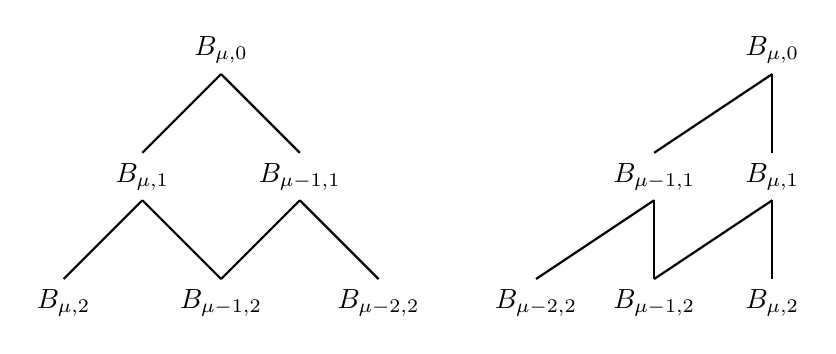
\begin{tikzpicture}[>=stealth, thick]

    % A box for "XAI" on the left
    \node (init) at (0,0) {$B_{\mu, 0}$};

    \draw (init.south) -- ++(-1, -1) coordinate (l);
    \draw (init.south) -- ++(1, -1) coordinate (r);

    \node[anchor=north] (l1) at (l) {$B_{\mu, 1}$};
    \node[anchor=north] (r1) at (r) {$B_{\mu - 1, 1}$};

    \draw (l1.south) -- ++(-1, -1) coordinate (l2);
    \draw (l1.south) -- ++(1, -1) coordinate (lr2);
    \draw (r1.south) -- (lr2);
    \draw (r1.south) -- ++(1, -1) coordinate (r2);

    \node[anchor=north] (l2) at (l2) {$B_{\mu, 2}$};
    \node[anchor=north] (lr2) at (lr2) {$B_{\mu - 1, 2}$};
    \node[anchor=north] (r2) at (r2) {$B_{\mu - 2, 2}$};

    \node (alt) at (7, 0) {$B_{\mu, 0}$};

    \draw (alt.south) -- ++(-1.5, -1) coordinate (altl);
    \draw (alt.south) -- ++(0, -1) coordinate (altr);

    \node[anchor=north] (altl1) at (altl) {$B_{\mu-1, 1}$};
    \node[anchor=north] (altr1) at (altr) {$B_{\mu, 1}$};

    \draw (altl1.south) -- ++(-1.5, -1) coordinate (altl2);
    \draw (altl1.south) -- ++(0, -1) coordinate (altr2);
    \draw (altr1.south) -- (altr2);
    \draw (altr1.south) -- ++(0, -1) coordinate (altr3);

    \node[anchor=north] (altl2) at (altl2) {$B_{\mu - 2, 2}$};
    \node[anchor=north] (altr2) at (altr2) {$B_{\mu - 1, 2}$};
    \node[anchor=north] (altr3) at (altr3) {$B_{\mu, 2}$};
\end{tikzpicture}